\documentclass[11pt,a4paper]{scrartcl}
\usepackage{setspace}
\usepackage{geometry}
\usepackage{hyperref}
\geometry{a4paper,tmargin=30mm,bmargin=30mm,lmargin=30mm,rmargin=30mm}
\usepackage[ngerman]{babel}

\usepackage[T1]{fontenc}      % T1-encoded fonts: auch Wörter mit Umlauten trennen
\usepackage[latin1]{inputenc}
\usepackage{currvita}

\usepackage{relsize}
\usepackage{soul}
\usepackage{xspace}


\usepackage[final]{graphicx}  % um Graphiken einzubinden
\usepackage{../picins} %fuer bild einfuegen


\newcommand{\ccplusplus}{{\sffamily\smaller C/{C}\hbox{\kern.05em\raise.25ex%
\hbox{+\kern-.01em+}\kern.05em}\spacefactor=1000 }}
\newcommand{\versal}[1]{\textsf{\textsmaller{\MakeUppercase{\caps{#1}}}}\xspace}

\newcommand*{\ac}[1]{\versal{#1}}
\tolerance=600

\renewcommand{\labelitemi}{$-$}
\renewcommand{\labelitemii}{$\bullet$}

\begin{document}
\parpic[rs][]{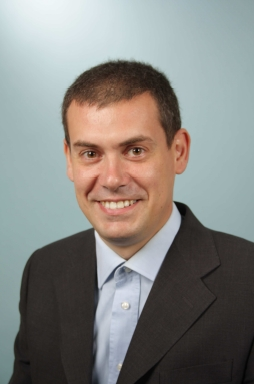
\includegraphics[width=3cm]{../Profilfoto.jpg}}
\begin{cv}{Curriculum Vitae}
\begin{cvlist}{Personal Data}
\item Dr. Michele Viti\\
Kirchenstra{\ss}e 9\\
22869 Schenefeld
\item Telefon: 040 53273453\\
Mobil: 0163 1903077\\
E"~Mail:~micheleviti78@gmail.com
\item Date of Birth: 17.\,April\,1978\\
Place of birth: Arezzo, Italy\\
Nationality: italian, german
\end{cvlist}

\begin{cvlist}{Work Experience}

\item[01.2010-today] Deutsches Elektronen-Synchrotron DESY Hamburg, researcher

{\scshape {\bfseries Projects:}}
\begin{description}
\item[04.2012-today] Development of the instrumentations for the electron bunch
control for the accellerator machines XFEL and FLASH I/II in DESY.
\item[06.2012-03.2015]Project PERCIVAL, Developement of a CMOS imaging
detector
\item[01.2010-05.2012]ALFA Project for ATLAS Experiment at CERN (Geneva,
Switzerland). Development and installation of tracking detector composed by
scintillating fibers  located in vacuum holders along the beam pipe at the LHC
accelerator
\end{description}
{\scshape {\bfseries Software:}}
\begin{description}
\item[Operating System] : Ubuntu Linux (12.04 und 16.04), Scientific Linux,
Windows XP/7
\item[Program Languages] : C++11, Python
\item[Software frameworks] : Qt, ChimeraTK, ROOT, Marlin
\item[SCADA] : DOOCS
\item[Communications Protocols] : TCP/IP, UDP
\item[Libraries] : GSL, ZMQ, boost, Minuit, HDF5
\item[Hardware] : MTCA Standard
\item[Version Control] : SVN, Git
\item[Integrated Development Environment] : Eclipse, Qt Creator
\end{description}

\vspace{\baselineskip}

\item[02.2005-01.2006] Perugia
University, Italy, researcher \\

Tasks:\\

Continuation of the masterthesis work.

\end{cvlist}

\begin{cvlist}{Doctoral Studies}
\item[02.2006-12.2009]

Deutsches Elektronen-Synchrotron DESY, Zeuthen, Linear Collider
Group.\\ Subject:
"`Precise and Fast Beam Energy Measurements at the International
Linear Collider"'

{\scshape {\bfseries Software:}}
\begin{description}
\item[Operating Systems] : Ubuntu Linux, Scientific Linux, Windows XP
\item[Program Languages] : C++, Python, Fotran
\item[Software frameworks] : GEANT 4, ROOT
\item[Libraries] : Minuit
\item[Monte Carlo Generators] : CAIN, COMRAD
\end{description}

\item[11.2009] PhD thesis defense

\end{cvlist}

\begin{cvlist}{Master Studies}
\item [11.1997-10.2004]Perugia University, Italy, Elementary Particle Physics.
Subject of the thesis:
"`Evaluation of a Tracking Algorithm for the Trigger of the KOPIO Experiment on the Decay
$K_L^0\rightarrow\pi^0\nu\bar{\nu}$"'\\

{\scshape {\bfseries Software:}}
\begin{description}
\item[Operating Systems] : Windows XP, Red Hat Linux
\item[Program Languages] : Fortran, C
\item[Software frameworks] : GEANT 3, PAW
\item[Libraries] : OpenGL
\end{description}
\end{cvlist}

\begin{cvlist}{High School}
\item[07.1997] Scientific High School Liceo Scientifico "`G. da
Castiglione"', Castiglion Fiorentino, Italy
\end{cvlist}

\begin{cvlist}{Leadership Positions}
\item [07.2011-05.2012] Coordinator of the Data Preparation Group for das ALFA
Project
%\begin{cvlist}{Weitere Qualifikationen}
%\item[06.2008] Specialized CERN Accelerator School "Beam Diagnostics", Dourdan, Frankreich
%\item[09.2010] Workshop ``Advanced Methods of Software Development'', Dresden
\end{cvlist}

\begin{cvlist}{Lehre}
\item [07.2006-02.2012] Supervision of DESY Summer students und
Master students
\item [02.2015] Internship in Grootmoor High School
\end{cvlist}

\begin{cvlist}{Business Stays Abroad}
\item [02.2006-12.2014] Living and working in Germany (since 12.2014 german
citizen).
\item [2006-2007] 5 periods of stay in Stanford University, USA
\item [02.2008] Nowosibirsk, Russian Federation
\item [01.2010-06.2012] Regular travels to Geneva, Switzerland
\end{cvlist}

\begin{cvlist}{Spoken Languages}
\item [Italian] native
\item [German] fluent
\item [English] fluent
\end{cvlist}

\begin{cvlist}{Weitere \ac{EDV} Knowledge}
%\item[Programmiersprachen] Pascal, \ac{BASIC}
\item[] \ac{MS OFFICE}, \ac{\LaTeX}, UML
\end{cvlist}

%\begin{cvlist}{Internal Notes}
%\item[] M.~Viti and S. Kostromin, Magnetic measurements for magnets
%  10D37, ILC-SLACESA TN-2008-1, 2008
%\end{cvlist}

\begin{cvlist}{Hobbies}
\item Sailing (Licenses: SBF Binnen, SBF See, SKS, SRC, UBI, FKN)
\item Crew member of the historical ship "`Zuversicht"', "`Verein
Jugendsegeln e.V."', Kiel
\item Club member Museumshafen \"Ovelg\"onne e.V., Hamburg
\item Hiking
\item Motorcycle
\item Low German Laguages
\end{cvlist}

%\begin{cvlist}{Publikationen}
%\item M. Viti, Precise and fast beam energy measurement at the
%  International Linear Collider, DESY-THESIS-2010-007
%  %\item M. Viti, Precise and Fast Beam Energy Measurement: Studies on the
%  % upstream beam energy monitors at the International Linear Collider,
%  % Suedwestdeutscher Verlag fuer Hochschulschriften, Juni 2010
%\item H.-J. Schreiber et al. (M.Viti) Magnetic measurements and simulations of
%  a 4-magnet dipole chicane for the International Linear Collider,
%  Particle Accelerator Conference (PAC07), Albuquerque, NM, U.S.A
%\item M. Viti, Energy measurement with Compton backscattering:
%  Updates, LCWS-2007-MDI23
%\item N. Muchnoi, H. J. Schreiber and M. Viti, ILC beam energy
%  measurement by means of laser Compton Backscattering,
%  Nucl. Instrum. Meth., A607:340-366, 2009
%\item A. Lyapin et al. (M.Viti) Results from a prototype chicane-based energy
%  spectrometer for a linear collider JINST 6 (2011) P02002,
%  arXiv:1011.0337
%\item M. Viti, Forward Physics Results from ATLAS, Hadron Structure
%  '11, Tatransk\'a \v{S}trba, Slovak Republic
%\item ATLAS authorship
%\end{cvlist}

\cvplace{Hamburg}
\date{\today}

\end{cv}

\end{document}
\endinput